\documentclass{workbook}

\coursenumber{MATH 16300}
\coursename{Sample Math Workbook Template}
\coursequarter{Spring 2026}
\instructorname{Subhadip Chowdhury}
\coverimage{images/sampleimage.png}
\department{Department of Mathematics}
\departmentlogo{images/sampleimage.png}
\addbibresource{references.bib}

\solutiontrue
\showplantrue

\begin{document}
\frontmatter
\maketitle

\PreTOCMatter{%
  {\Huge\bfseries A Repository-Style Minimal Working Example}\par
  \vspace{1em}
  This page is inserted with \texttt{\string\PreTOCMatter}. It is useful for a short note,
  dedication, or instructor-facing cover page before the table of contents.
}

\epigraph{Mathematics, rightly viewed, possesses not only truth, but supreme beauty.\\[0.5em]
\hfill --- Bertrand Russell}
\makeepigraph

\tableofcontents

\FrontMatter{How to Use This Template}
This repository demonstrates workbook mode in \texttt{main.tex} and worksheet mode in
\texttt{assignments/assignment1.tex} and \texttt{assignments/assignment2.tex}. The workbook includes
chapter files from \texttt{chapters/} and appendix files from \texttt{appendices/}. It also cites a few
sample references such as \cite{apostol-calculus,axler-linear} and uses a placeholder image stored at
\texttt{images/sampleimage.png}.

\FrontMatter{Introduction}
This introduction shows the workbook voice and layout. The class provides convenient color-switching
macros such as {\blue blue text}, {\maroon maroon text}, and {\lake lake-colored text}. It also
provides an emphasis macro: \alert{important ideas can be highlighted consistently}. Throughout the
template, cross-references use \verb|\cref|, for example \cref{thm:derivative-power,def:inner-product}.

\begin{center}
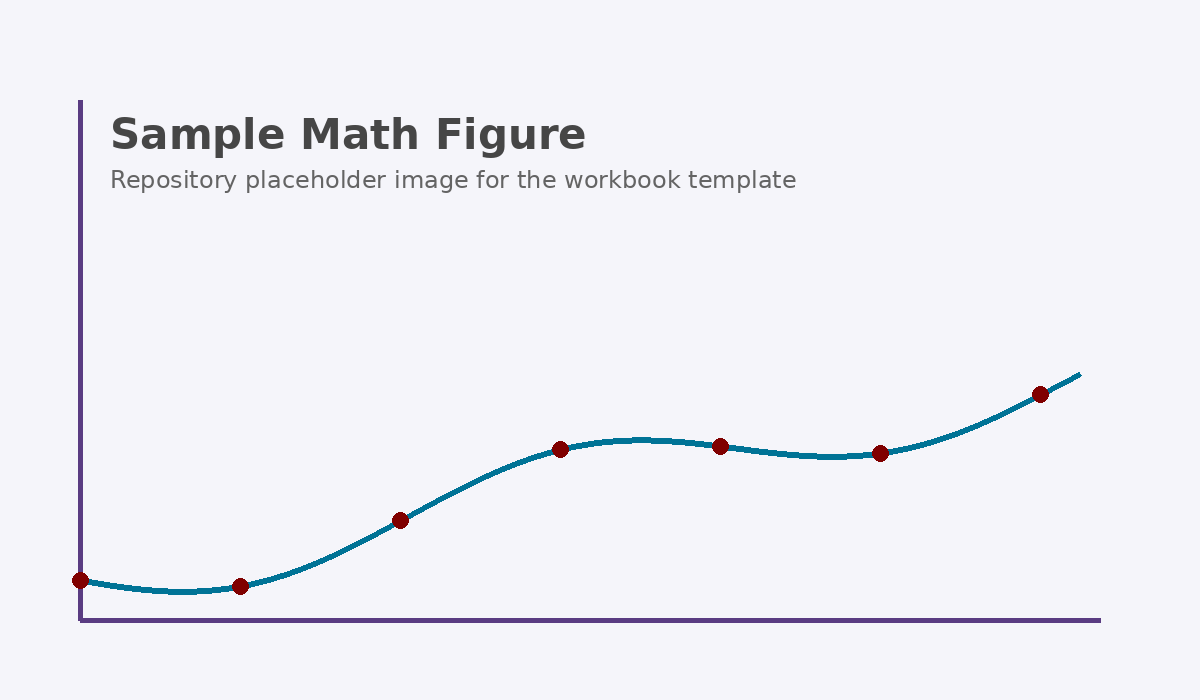
\includegraphics[width=0.55\linewidth]{images/sampleimage.png}
\end{center}

\chapterline{maroon}{88}

\section{Repository structure}
The top-level file \texttt{main.tex} compiles the workbook. The folder \texttt{chapters/} stores modular
chapter files, \texttt{appendices/} stores appendices, and \texttt{assignments/} stores standalone
worksheet-mode assignments. The command \verb|\blankfill| is useful for fill-in-the-blank prompts:
Course website \blankfill

\begin{note}[Template note:]
This note box shows one recommended use of the class: keep exposition in workbook mode and use the
worksheet option for short assignments or handouts.
\end{note}

\begin{warning}[Compilation reminder:]
Because the class uses \texttt{biblatex} with the \texttt{biber} backend, the workbook should be compiled
with a LaTeX $\to$ Biber $\to$ LaTeX $\to$ LaTeX workflow.
\end{warning}

\begin{digression}
A compact workbook often benefits from short historical or conceptual side paths. This environment is a
natural place to discuss why a result matters before returning to the main thread.
\end{digression}

\begin{lectureplan}[Opening module]
\planhead{Learning Objectives}
Students should recognize the repository layout, identify the main entry points, and understand how the
class structures theorem-like environments.

\planhead{Timing (10 minutes)}
Spend a few minutes walking through the folder structure and the sample chapter files.
\end{lectureplan}

\begin{staffnote}[Instructor note:]
The lecture-plan and staff-note environments are most useful in instructor-facing copies of the workbook.
Set \texttt{\string\showplanfalse} in a student-facing version if you want to suppress them.
\end{staffnote}



\mainmatter

\include{chapters/chapter1}
\include{chapters/chapter2}

\appendix
\chapter{Appendix: Cross-References and Citations}

This appendix exists mainly to show that the workbook can cite references from a shared
\texttt{references.bib} file. For example, a standard calculus text is \cite{apostol-calculus}, while a
clean linear algebra text is \cite{axler-linear}.

\begin{note}[Cross-reference example:]
Earlier we introduced \cref{def:inner-product}, proved \cref{thm:derivative-power}, and used
\cref{ex:derivative} as a worked example.
\end{note}

\section{First Section}
\begin{theo}{}
    Sample theorem.
\end{theo}

\begin{exercise}[Reflection]
Write two sentences explaining how you would adapt this repository for a quarter-long course.
\myskip
\end{exercise}

\chapter{Appendix: Worksheet Files in the Repository}

The files \texttt{assignments/assignment1.tex} and \texttt{assignments/assignment2.tex} are standalone
worksheet documents using the \texttt{worksheet} option. They show how to keep handouts separate from
\texttt{main.tex} while still sharing the same class file and macro vocabulary.

\begin{warning}[GitHub tip:]
When you upload this repository, it is helpful to include a short README that explains which files compile
independently and which files are included only through \texttt{main.tex}.
\end{warning}

\begin{digression}
A modular folder structure makes it much easier to reuse notation, styling, and reference data across a
whole sequence of lecture notes and assignments.
\end{digression}


\backmatter
\makebibliography

\end{document}
